\begin{figure}[H]
  \centering
  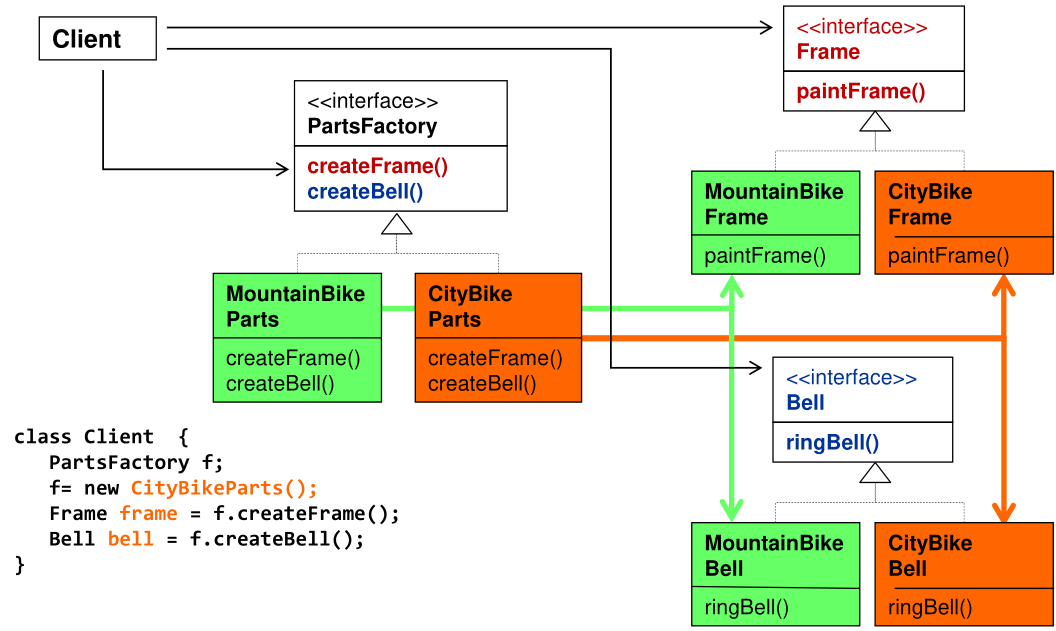
\includegraphics[width=1.0\columnwidth]{figures/abstractFactory.png}
\end{figure}
\begin{intentbox}[Intent]\\
Provide an interface for creating families of related or dependent objects without specifying their concrete classes.\\
  \rdb{Abstract Factory}=\rdb{Abstract Method}+\rdb{Strategy Pattern}\\
\end{intentbox}
\begin{partbox}\nospacing
  \begin{itemizenosep}
      \item \imp{Abstract/Interface Factory}: declares methods in order to
    create products of a certain family by:
    \begin{itemize}
        \item declaring an interface operations that create abstract products.
      \begin{mintlinebox}{java}
        interface Factory{
          intA createA();
          intB createB();
       }  
      \end{mintlinebox}
        \item declaring an abstract class that provides methods to produce
      abstract products
      \begin{mintlinebox}{java}
        abstract class Factory{
          public abstract intA createA();
          public abstract intB createB();
        }
      \end{mintlinebox}
    \end{itemize}
    $\Rightarrow$ methods to create product must share common interface:
    \begin{mintlinebox}{java}
      intA createProdA();
    \end{mintlinebox}
      \item \imp{Concrete Factories}: implements operations to create concrete
    products.
      \item \imp{Abstract/Interface Product}: declares an interface for a type
    of product. 
      \item \imp{Concrete Products}: products to be created by the corresponding
    ConcreteFactory;\\
    Need to implement the corresponding product interface in order to be
    consistent with the factories.
      \item \imp{Client}: Uses a factory in order to obtain products of a
    certain family.\\
    \imp{Note}: this may 
  \end{itemizenosep}
\end{partbox}
\subsubsection{Where is the concrete Factory}
\begin{sectionbox}\nospacing
 \begin{itemize}
     \item Directly used by client
     \item by another class that uses e.g.\ factory method and singleton 
 \end{itemize} 
\subsubsection{Who creates the concrete factory?}
\end{sectionbox}
\begin{itemizenosep}
    \item \imp{Externally}:
  \begin{mintlinebox}{java}
		CurrentFactory.setFactory(new Factory1());
  \end{mintlinebox}
    \item \imp{Internally}:
  \begin{mintlinebox}{java}
		CurrentFactory.setFactory(new Factory1());
  \end{mintlinebox}
    \item \imp{Automatically upon loading}:
  \begin{mintlinebox}{java}
		class Factory1 implements Factory {
      public A createA() { ... }
      public B createB() { ... }
      static {
        CurrentFactory.setFactory(new Factory1());
      }
      private Factory1() { };
    }
  \end{mintlinebox}
\end{itemizenosep}
\begin{defnbox}\nospacing
  \begin{defn}[Static Block]\label{defn:staticBlock}
    Will be called only once at initialization even-though if we call the
    constructor multiple times.
  \end{defn}
\end{defnbox}
\subsubsection{Difference factory Method and abstractFactory}
\begin{sectionbox}\nospacing
  The main difference between a "factory method" and an "abstract factory" is that the factory method is a single method, and an abstract factory is an object. I think a lot of people get these two terms confused, and start using them interchangeably. I remember that I had a hard time finding exactly what the difference was when I learnt them.
\end{sectionbox}
\begin{sectionbox}[Factory Method Paradigm]\nospacing
  \ldots the Factory Method pattern uses inheritance and relies on a subclass to
  handle the desired object instantiation.
\end{sectionbox}
\begin{sectionbox}[Abstract Factory Paradigm]\nospacing
  With the Abstract Factory pattern, a class delegates the responsibility of
  object instantiation to another object via composition.\\
  What they're saying is that there is an object A, who wants to make a Foo object. Instead of making the Foo object itself (e.g., with a factory method), it's going to get a different object (the abstract factory) to create the Foo object.
\end{sectionbox}
\begin{notebox}[Factory vs. DI]\nospacing
  When using a factory your code is still actually responsible for creating objects. By DI you outsource that responsibility to another class or a framework, which is separate from your code.
\end{notebox}
%%% Local Variables:
%%% mode: latex
%%% TeX-master: "../formulary"
%%% End:
